
\documentclass{article}
\usepackage[letterpaper,top=0.5in,bottom=0.5in,left=.5in,right=.5in,includeheadfoot]{geometry}
\usepackage{amssymb,amsmath}
\usepackage{parskip}
\usepackage{fancyhdr}
\usepackage{tabu}
\usepackage{enumerate}
\usepackage{graphicx}
\usepackage{tikz}
\usepackage{multicol}
\usepackage{color}
\usepackage{soul}
\usepackage{changepage}
\usepackage{endnotes}
% \usepackage{dblfnote}
\usepackage{hyperref}
\hypersetup{colorlinks=true,urlcolor=blue}

\renewcommand{\baselinestretch}{1.3}
\pagestyle{fancy}
\fancyfoot{}
\renewcommand{\headrulewidth}{0pt}
\setlength{\headheight}{0pt}

\fancypagestyle{firstpage}{
  \fancyhead{}
  \fancyfoot{}
}

\usepackage{titlesec}

\titlespacing\title{0pt}{0pt plus 4pt minus 2pt}{-5pt plus 2pt minus 2pt}
\titlespacing\section{0pt}{-8pt plus 4pt minus 2pt}{-6pt plus 2pt minus 2pt}
\titlespacing\subsection{0pt}{0pt plus 4pt minus 2pt}{-6pt plus 2pt minus 2pt}
\titlespacing\subsubsection{0pt}{0pt plus 4pt minus 2pt}{-5pt plus 2pt minus 2pt}


\newcommand{\TODO}{\textcolor{red}{\textbf{\hl{TODO}}}}

\begin{document}
% \thispagestyle{firstpage}
% \PrintFirstHeader{}
% \pagebreak


%================================ COVER PAGE ================================

%*********** Use this for project proposal (comment out in project report) ************
\emph{\footnotesize{CIS 520 Spring 2019, Project Report}}

%*********** Use this for project report (comment out in project proposal) ************
%\emph{\footnotesize{CIS 520 Spring 2018, Project Report}}

\vspace{12pt}

%Fill in your project title
\textbf{\Large{Project Title}}

\vspace{1cm}

\textbf{Team Members:} \\
%Fill in your team details; remove any lines that are not needed
Monal Garg (PennKey: \texttt{mgarg}; Email: \texttt{mgarg@sas.upenn.edu}) \\
Amit Gupta (PennKey: \texttt{akgupta}; Email: \texttt{akgupta@seas.upenn.edu}) \\
Aashish Jain (PennKey: \texttt{aashj99}; Email: \texttt{aashj99@seas.upenn.edu}) \\
Moksh Jawa (PennKey: \texttt{moksh}; Email: \texttt{moksh@seas.upenn.edu})

%---

\vspace{2cm}

%*********** Comment out the following for the proposal; uncomment and fill in all details for the project report ***********

\textbf{Assigned Project Mentor:}

%Fill in assigned TA name
Jane Lee

\vspace{1cm}

\textbf{Team Member Contributions:}

%Fill in team member contributions
\begin{center}
\begin{tabular}{|l|l|}
\hline
Team Member & Contributions \\
\hline
Monal Garg & Past Work, Solution Approach, Machine Learning Algorithms, Visualizations, Report \\
  & (continue if needed) \\
\hline
Amit Gupta & Problem Formulation, Algorithms Plan for Use, Machine Learning Algorithms, Visualizations, Report \\
  & (continue if needed) \\
\hline
Aashish Jain & Data Cleaning, Data Stitching, Machine Learning Algorithms, Visualizations, Report \\
  & (continue if needed) \\
\hline
Moksh Jawa & Data Cleaning, Data Stitching, Machine Learning Algorithms, Visualizations, Report \\
  & (continue if needed) \\
\hline
\end{tabular}
\end{center}

\vspace{12pt}

\textbf{Code Submission:}

\normalsize{Public GitHub Repo can be found at \href{https://github.com/akgpta/CIS520-Final-Project}{https://github.com/akgpta/CIS520-Final-Project}}



\newpage
\tableofcontents
\newpage

\section{Abstract}
Suicide is a major public health concern worldwide. Because living in a different countries and therefore different environment can greatly impact one's lifestyle, we wanted to explore suicide rates over various countries. Specifically, we considered $78$ countries over the five years from $2010$ to $2014$. For each country, we collected data on ground truth suicide rates, Youth Unemployment, Alcohol Consumption, Life Expectancy, Country Population, and Fertility Rate. We were interested in understanding how these factors could help predict suicide rates. To do this, we implemented $k$-Nearest Neighbors, Linear Regression, and Neural Networks. Results can be best summarized as the data fully characterize the problem. What we mean is that the countries seem to have an endogenous suicide rate, but that is determined outside of our input features. However, our features are complex enough to identify countries with this information and map it to the suicide rates. This gives an essentially overfit model which actually performs well due to high time correlation of suicide rates per country through time. 

\begin{multicols}{2}
\section{Introduction}
\subsection{Problem Motivation} Unfortunately, it is a sad reality that many individuals each year commit suicide. We in the U.S. are slowly being aware of this issue, but we wanted to understand suicide rates internationally. Especially, we wanted to look at these rates as they related to common features of each country, such as GDP, unemployment, and alcohol consumption. At a high-level we wanted to draw out any meaningful relationship between these macro features and suicide rates.
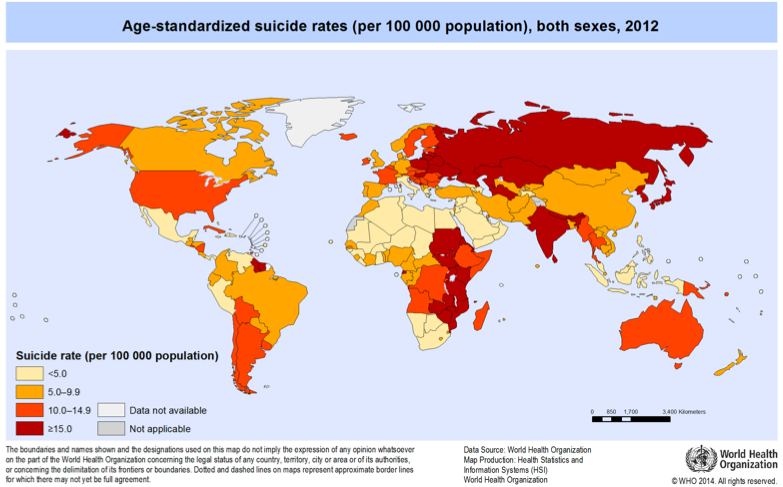
\includegraphics[width=\columnwidth]{2012-data-vis-map.png}
\subsection{Data Set and Source} Our project grew from an intriguing 
World Health Organization data set will well over 35 years of suicide rates by country broken up by demographics.  \endnote{https://www.kaggle.com/szamil/who-suicide-statistics}. In an effort to extend existing analyses though, we actually sources global data from a variety of sources. This included a FiveThirtyEight data set on alcohol consumptixon \endnote{https://www.kaggle.com/fivethirtyeight/fivethirtyeight-alcohol-consumption-dataset}. We also incorporated a World Bank Data Set on Youth Unemployment \endnote{https://www.kaggle.com/sovannt/world-bank-youth-unemployment} and another from the World Bank on population, fertility, and life expectancy \endnote{https://www.kaggle.com/gemartin/world-bank-data-1960-to-2016}. A lot of the work done was with respect to time series and things like that. What we wanted to do, though, was take a look at combining data from multiple sources. 
Our project team sought to understand a little bit more about the intricacies of sourcing data from multiple places. This proved to be a difficult challenge.  
\subsection{Summary Statistics} 
We've provided summary statistics for 4 of the datasets we will be using in our project shown in Tables \hyperref[summary-statistic-table-alcohol]{0}, \ref{summary-statistic-table-youth-unemployment}, \ref{summary-statistic-table-fertility}, \ref{summary-statistic-table-life}, some of which are located in the appendix.

\begin{adjustwidth}{8px}{}
\begin{tabular}{|l|l|}
\hline
Statistic          & Average liters/person/year \\ \hline
Min                & 0                          \\ \hline
Max                & 14.4                       \\ \hline
Mean               & 4.71                       \\ \hline
Median             & 4.2                        \\ \hline
Standard Deviation & 3.77                       \\ \hline
\multicolumn{2}{c}{Table 0: Alcohol Consumption by Country} 
\label{summary-statistic-table-alcohol}
\end{tabular}
\end{adjustwidth}


\section{Related Work}
\subsection{Related to Models} 

Among the papers that analzyed economic factors, a regression model seemed to be the popular choice of method. For example, Pandey and Kaur paper used a Auto-Regressive Distributed Lag (ARDL) model \endnote{https://crawford.anu.edu.au/acde/asarc/pdf/papers/2009/WP2009/{\_}08.pdf}. 

Most of the articles concerning the relationship of suicide rate and alcohol consumption related trends from a biological perspective utilized relatively simple statistical analysis \endnote{https://www.ncbi.nlm.nih.gov/pubmed/9229027}. Whereas medical research that involved more complex forms of data such as fMRI brain scans utilized algorithms such as Gaussian Naive Bayes \endnote{https://nocklab.fas.harvard.edu/files/nocklab/files/just{\_}2017{\_}machlearn{\_}suicide{\_}emotion{\_}youth.pdf}.

\subsection{Related to Problem} 

During our research, we came across multiple research papers that analyze the correlation between suicide rates and either economical, behavioral, medical, or psychological factors. For example, the Pandey and Kaur paper investigates suicidal trend and economic determinants in an Indian population\endnote{https://crawford.anu.edu.au/acde/asarc/pdf/papers/2009/WP2009/{\_}08.pdf}. Whereas articles published in medical journals explored suicide with alochol/drug consumption, psychotic behavior, brain scans, etc \endnote{https://www.ncbi.nlm.nih.gov/pmc/articles/PMC2872355/}. 

However, most papers tend to focus on either the economic or behavioral/medical factors. As suicide is likely governed by multiple factors, we seek to investigate this problem through a more holistic approach by simultaneously analyzing both medical, behavioral, and economic factors. Through this application of machine learning, we hope to gain insight on the relative role each factor plays in suicide and about the interaction of these factors. 

Moreover, most papers perform a time series analysis. We provide a different approach by analyzing the data by country. Papers that do focus on certain regions usually provide analyses on one country or a specific region, whereas we will analyze global statistics. 


\section{Problem Formulation and Data} 
\subsection{Data Processing Needed} Our data came in a variety of comma-separated formats. A lot of countries were labelled in differing manner and years were often a column and other times a point in a row. We used Excel Pivot Tables to make the CSVs more easily parsable and standardized. Later, we used Pandas and Python to remove blanks and other issues with inconsistencies and finish with an aggregated set of data. Other pre-processing includes filling in missing values, reconciling some country names such as (Trinidad \& Tobago vs. Trinidad and Tobago), and dropping some values if a country was not universal across all CSVs. Our final product was a single CSV with 78 rows (countries) with columns for each of the 8 features. The relatively small number of countries is a testament to the variance in countries in each dataset as well as the missing values.
\subsection{Inputs, Outputs} Inputs are a variety of real-valued data points tied to the country. They are described above. Most are also measured for a specific year, however some are just duplicated across all years (e.g. Alcohol Consumption). Such data points were simply treated as constant for a country through time. We threw out examples which were missing features our true values. Outputs are a model, which given a countries characteristic features, can predict suicide rates. 
\subsection{Performance Measures} Given the regression nature of this problem, we used squared loss model to measure our performance. This is because with positive real valued data with explicit bounds of $[0, 10^5]$, but more reasonable empirical bounds of around $[0, 10^3]$. The following image is a representation of squared loss,but in a one dimensional feature space \endnote{https://blog.algorithmia.com/introduction-to-loss-functions/.}
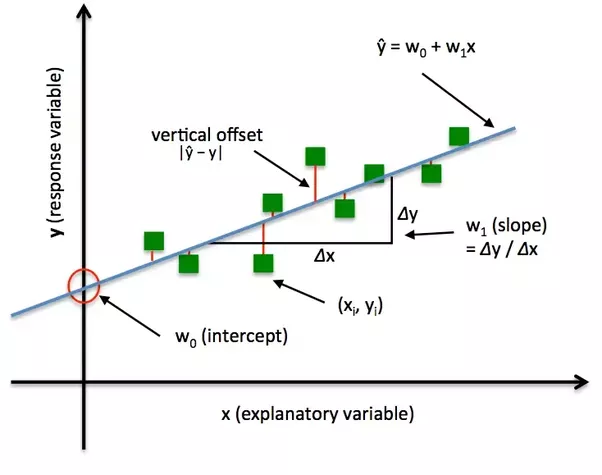
\includegraphics[width=\columnwidth]{squared-loss.png}


\section{Methods and Results}
\subsection{Experiment Set Up} Altogether, we had five years worth of data on $78$ countries. We maintained the same training data, test data, and folds when implementing all three types of models. The data from 2014 data was reserved as the test data and we trained our models on the data from $2010$ to $2013$. Four folds were set up that such that each one reserved a different year from the $2010$ to $2013$ data to test with. 

\subsection{k Nearest-Neighbors} We first implemented a $k$-nearest neighbor algorithm using Euclidean distance as we suspected suicide rates between similar countries would be comparable. We cross validated across the following values of $k = [1,2, 3, 4, 5, 6, 7, 8, 9, 10]$ and found that $k = 1$ produced the best model with a cross validation squared error of $4.697 * 10^4$, training error of $8.160 * 10^6$ and test error of $1.720 * 10^6$. Although this error appears to be high, we remind the reader that this squared error is taken over $78$ test data points and each of the suicide rate values can be as large as $10000$. 

The graph below shows the results when cross-validating over different $k$ values. Here we have omitted the training and test error to highlight an interesting trend in cross-validation error. Recall that our each of our folds have data of from each country of $3$ years. Say we are looking for the nearest neighbors for country $x$. We suspect that the error is very low for $k$ values of $1, 2, 3$ because the model is utilizing the country $x$'s $3$ data points from different years to predict suicide rates for the test year. Errors then pick up for values of $k$ greater than $3$ because the model is forced to use the data from countries other than country $x$, which may not be as informative when making decision about suicide rates for country $x$. 

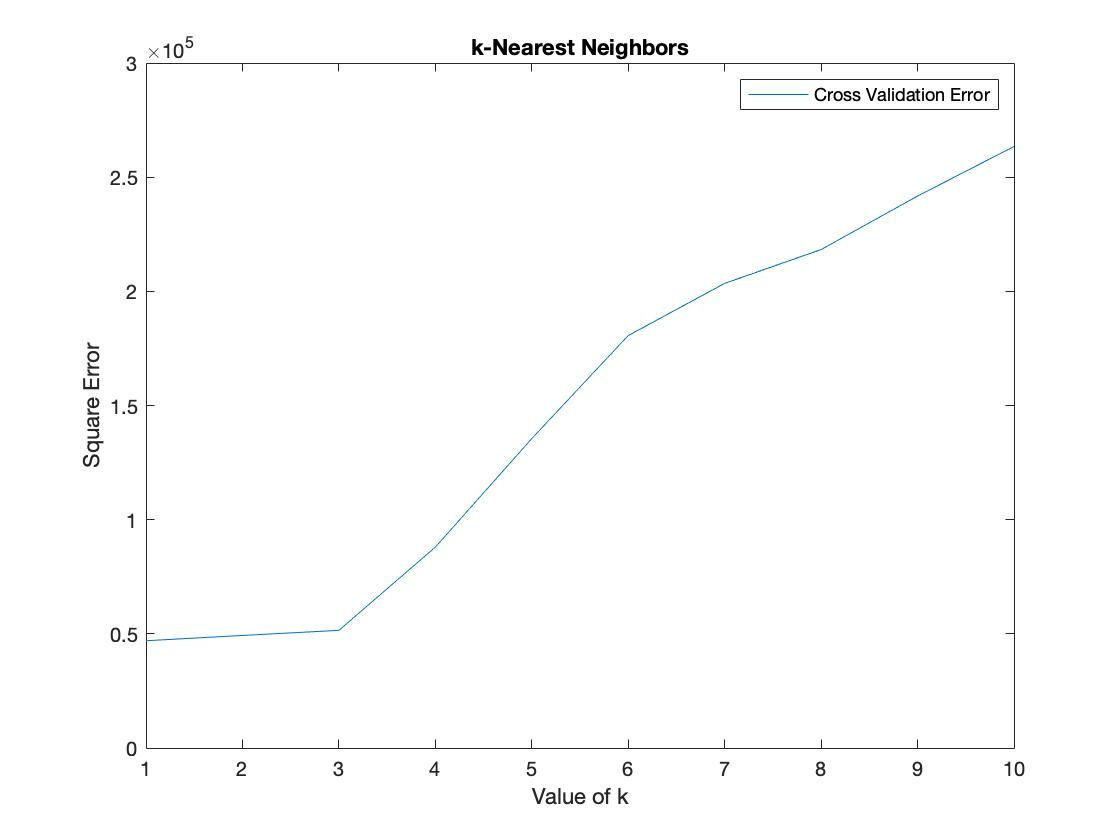
\includegraphics[width=\columnwidth]{../Figures/k_nn_cv_err.jpg}

To take this a step further, we also built a near neighbor model using Minkowski's distance, a more general distance formula, shown below.

\[D\left(\mathbf{x}_{i}, \mathbf{x}_{j}\right)=\left(\sum_{l=1}^{d}\left|x_{i l}-x_{j l}\right|^{q}\right)^{1/q}\]

We cross validated across the following values of $q = [1, 2, 3, 4, 5]$ and for each of these $q$ values, found the best $k$ value. Interestingly, we found for each value of $q$, $k = 1$ produced the minimum squared error. Moreover, the same phenomenon of small errors for $k$ values from one to tree and relatively larger errors for every subsequent value of $k$ was observed for all values of $q$. Overall, $k = 1$ and $q = 2$ (which is equivalent to Euclidean distance) produced the best model.

\includegraphics[width=\columnwidth]{../Figures/k-nn-err-cv-minkowski.jpg}

\subsection{Neural Network} \TODO(Aashish) Ran neural net on $1$ hidden network...

\subsection{Linear Regression} First, we implemented a linear regression as our base line model. 


A most related papers ran linear regression, we also ran regularized and unregularized least squares linear regression to see if perhaps we could prevent this overfitting. This is our base line model \TODO(maybe say excessive details are left out for the sake of parsimony?) \TODO 

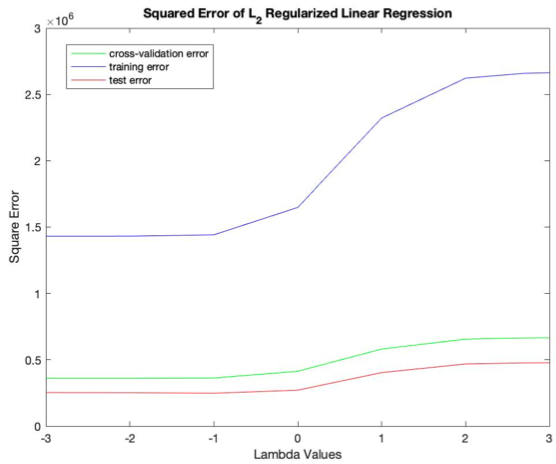
\includegraphics[width=\columnwidth]{lin_reg.png}

\subsection{Results}

When we ran neural net with 1 hidden layer, we saw that our model only got better as the model’s complexity increased, further showing that our model was essentially grossly overfitting to the train data and essentially functioning as a memorizer.
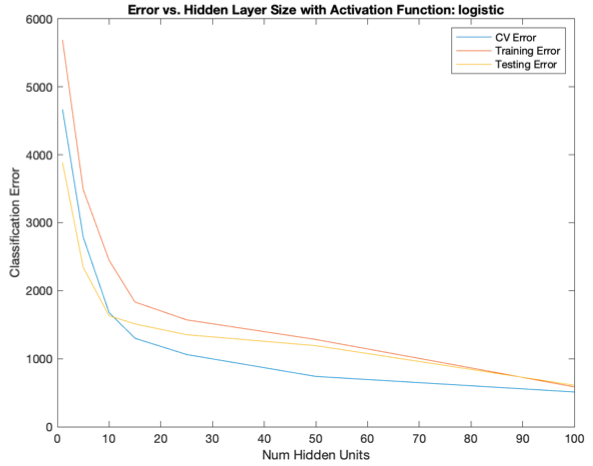
\includegraphics[width=\columnwidth]{neur-net.png}


\includegraphics[width=\columnwidth]{geo-bee.jpg}
The best predictor of suicide rates is the country label itself. Suicide rates in Ghana in 2013 are going to look like suicide rates in Ghana in 2012 most. Modelling this regression outcome as independent draws disregards the time series data and correlation of examples. As such, nearest neighbors performs exceptionally well, since it just recognized the country through these 8 input features. 

\section{Discussion and Reflections}

We see a lot of what would canonically be overfitting in the data. However, in the context of this problem overfitting is not necessarily the worst. We have such complete data that we can actually begin to drive at the underlying distribution at a per instance level. Note, when we say instance here we are referring to a unique country (not a specific $R^8$ vector in the input space). This means our classifiers actually easily approach a Bayes Optimal Classifier. \\
We recall the handwriting recognition problem from class. Consider fitting a unique model to an individual with fairly comprehensive handwriting samples. Handwriting for an individual evolves very minimally over time and there really are only 26 letters. Overfitting and understanding what exactly these 26 letters look like in some sort of training set for the individual means that predictions of future handwriting \textit{for that individual} will be fairly reliable. \\
This project was certainly an adventure in machine learning. Let us recall some of the lines from what we set out to do. Note, these were established a priori in our proposal: \textit{``at a high-level we wanted to draw out any meaningful relationship between these macro features and suicide rates'}' and \textit{``we hope to gain insight on the
relative role each factor plays in suicide and about the interaction of these factors''}. We were thinking that a model would illimuniate which features wre coupled with suicide rates. As the project continued though, as noted in our Results section, models were essentially using the features to identify individual countries. We are careful in this report to not conflate correlation with causation and, as such, have left out implications of this country-recognizer model built. \\
Reflecting on our goal, it seems the problem we have chosen to tackle doesn't really make sense from a machine learning perspective. Sure, the factors we have chosen can be used to generate a model which fairly reliably outputs suicide rates. However, this correlation should not be taken to imply causation or even anything close to that. From a model story perspective, suicide rates are affected by many factors exogenous to our world of data but endogenous to a country. \\
When you consider some sort of underlying sampling distribution assumptions on the data, it doesn't make sense that suicide rates for countries on different continents with different socioeconomic statuses are coming from one distribution. Although this seems to say that this project wasn't an effective learning opportunity, we as a team feel quite the opposite. \\
There are a finite number of countries in the world. In fact, there are 195 countries in the world. As such, worries about reasonable time computation, tractability, and other aspects of problems centered on larger data (think users of Netflix or game states) does not really factor in here. Had we as a group had more experience at the start of this project, perhaps we would have foreseen the uniqueness of countries leading to a model which could basically be a geography bee champion. However, we feel that the machine learning exercises carried out during the course of this project deepened our understanding of course algorithms, implications, and relevant considerations.




% \subsection{Pre-Milestone Meeting Goals} 

% Our goal before our milestone meeting is have the data completed clean and visualized. Additionally, we plan to have k-Nearest Neighbors and Least Squares Regression implemented, visualized, and results recorded. Note that our k-Nearest Neighbor implementation will have weighted scaling based on features rather than Euclidean distance.

% \subsection{Timelines}

% After our milestone meeting, we will have exactly 3 weeks. The first week will involve implementing our last approach of decision stubs as features and feeding them into neural nets. The second week will involve finetuning and evaluating our models. The last week will be for writing up the report

\section{Acknowledgements} First and foremost, we would like to acknowledge our project mentor, Jane Lee, for being very helpful throughout the project and Professor Agarwal for a fantastic class. Additionally, we acknowledge the Kaggle users who provided the datasets.

\end{multicols}

\pagebreak

\section{References} \theendnotes

\section{Appendix} 
\begin{table}[ht]
\centering
\begin{tabular}{|l|l|l|l|l|l|}
\hline
          &  \multicolumn{5}{c|}{Youth Unemployed} \\ \hline
Statistic          &  \%  2010 &  \% 2011 &  \% 2012 &  \%  2013 & \% 2014 \\ \hline
Min                & 0.6999                    & 0.6999                    & 0.5                       & 0.6999                    & 0.6999                    \\ \hline
Max                & 57.2                      & 57.1                      & 61.7                      & 58                        & 57.9                      \\ \hline
Mean               & 17.89                     & 17.9                      & 18.15                     & 18.1                      & 17.94                     \\ \hline
Median             & 14.9                      & 14.52                     & 14.4                      & 14.1                      & 14.12                     \\ \hline
Standard Deviation & 10.54                     & 10.88                     & 11.43                     & 11.67                     & 11.55                     \\ \hline
\end{tabular}
\caption{Youth Unemployment by Country}
\label{summary-statistic-table-youth-unemployment}
\end{table}
\begin{table}[ht]
\centering
\begin{tabular}{|l|l|l|l|l|l|}
\hline
          &  \multicolumn{5}{c|}{Fertility Rates} \\ \hline
Statistic          &  \%  2010 &  \% 2011 &  \% 2012 &  \%  2013 & \% 2014 \\ \hline
Min                & 1.06                   & 1.11                   & 1.16                   & 1.13                   & 1.21                   \\ \hline
Max                & 7.49                   & 7.46                   & 7.42                   & 7.38                   & 7.34                   \\ \hline
Mean               & 2.91                   & 2.88                   & 2.84                   & 2.81                   & 2.79                   \\ \hline
Median             & 2.41                   & 2.37                   & 2.34                   & 2.34                   & 2.33                   \\ \hline
Standard Deviation & 1.45                   & 1.42                   & 1.39                   & 1.37                   & 1.34                   \\ \hline
\end{tabular}
\caption{Fertility Rates by Country}
\label{summary-statistic-table-fertility}
\end{table}
\begin{multicols}{2}


\end{multicols}
\begin{table}[ht]
\centering
\begin{tabular}{|l|l|l|l|l|l|}
\hline
          &  \multicolumn{5}{c|}{Life Expectancy} \\ \hline
Statistic          &  \%  2010 &  \% 2011 &  \% 2012 &  \%  2013 & \% 2014 \\ \hline
Min                & 47.56                  & 48.284                 & 49.041                 & 49.825                 & 50.621                 \\ \hline
Max                & 82.9780488             & 83.4219512             & 85.4170732             & 83.8317073             & 83.9804878             \\ \hline
Median             & 72.2783848             & 72.4719847             & 72.657                 & 72.786                 & 72.9707317             \\ \hline
Standard Deviation & 8.34929356             & 8.19102272             & 8.04819537             & 7.89104622             & 7.80484223             \\ \hline
\end{tabular}
\caption{Life Expectancy by Country}
\label{summary-statistic-table-life}
\end{table}





\end{document}
